\documentclass[10pt,conference]{IEEEtran}
\IEEEoverridecommandlockouts

\usepackage{cite}
\usepackage{amsmath,amssymb,amsfonts}
\usepackage{algorithmic}
\usepackage{graphicx}
\usepackage{textcomp}
\usepackage{xcolor}
\usepackage{listings}

% load macros
% Scala code style
\definecolor{dkgreen}{rgb}{0,0.6,0}
\definecolor{gray}{rgb}{0.5,0.5,0.5}
\definecolor{mauve}{rgb}{0.58,0,0.82}
\lstdefinestyle{myScalastyle}{
  frame=tb,
  language=scala,
  aboveskip=3mm,
  belowskip=3mm,
  showstringspaces=false,
  columns=fixed,
  basicstyle={\footnotesize\ttfamily},
  numbers=none,
  keywordstyle=\color{blue},
  commentstyle=\color{dkgreen},
  stringstyle=\color{mauve},
  frame=single,
  breaklines=true,
  breakatwhitespace=true,
  tabsize=3,
}
\lstdefinestyle{smallScalastyle}{
  frame=tb,
  language=scala,
  aboveskip=3mm,
  belowskip=3mm,
  showstringspaces=false,
  columns=fixed,
  basicstyle={\scriptsize\ttfamily},
  numbers=none,
  keywordstyle=\color{blue},
  commentstyle=\color{dkgreen},
  stringstyle=\color{mauve},
  frame=single,
  breaklines=true,
  breakatwhitespace=true,
  tabsize=3,
}

% ECMAScript Intermediate Reprentations
\lstdefinestyle{ires}{
  frame=tb,
  aboveskip=3mm,
  belowskip=3mm,
  showstringspaces=false,
  columns=fixed,
  basicstyle={\footnotesize\ttfamily},
  numbers=none,
  keywordstyle=\color{blue},
  commentstyle=\color{dkgreen},
  stringstyle=\color{mauve},
  frame=single,
  breaklines=true,
  breakatwhitespace=true,
  tabsize=3,
}

% JavaScript code style
\lstdefinelanguage{JavaScript}{
  keywords={async, await, break, case, catch, class, const, continue, debugger,
    default, delete, do, else, enum, export, extends, false, finally, for,
    function, if, import, in, instanceof, new, null, return, super, switch, this,
    throw, true, try, typeof, var, void, while, with, yield},
  keywordstyle=\color{blue}\bfseries,
  ndkeywordstyle=\color{darkgray}\bfseries,
  identifierstyle=\color{black},
  sensitive=false,
  comment=[l]{//},
  morecomment=[s]{/*}{*/},
  commentstyle=\color{purple}\ttfamily,
  stringstyle=\color{red}\ttfamily,
  morestring=[b]',
  morestring=[b]"
}

\lstdefinestyle{myJSstyle}{
  language=JavaScript,
  extendedchars=true,
  basicstyle=\footnotesize\ttfamily,
  showstringspaces=false,
  showspaces=false,
  numbers=none,
  tabsize=2,
  breaklines=true,
  showtabs=false,
  captionpos=b
}

% thicker vertical line
\newcolumntype{?}{!{\vrule width 1pt}}

% names
\newcommand{\cfg}{\text{CFG}}
\newcommand{\bnf}{\text{BNF}}
\newcommand{\es}{\text{ES}}
\newcommand{\bnfes}{\bnf_\es}
\newcommand{\peg}{\text{PEG}}

% codes
\newcommand{\code}[1]{\text{\lstinline[style=myJSstyle]!#1!}}
\newcommand{\kwtrue}{\code{true}}
\newcommand{\kwt}{\code{\#t}}
\newcommand{\kwfalse}{\code{false}}
\newcommand{\kwf}{\code{\#f}}

%BNF_ES
\newcommand{\symb}{s}
\newcommand{\NT}[1]{#1}
\newcommand{\T}[1]{\code{#1}}
\newcommand{\argument}{a}
\newcommand{\param}{p}
\newcommand{\butnot}{\!\smallsetminus\!}
\newcommand{\rhs}{\alpha}
\newcommand{\cond}{c}
\newcommand{\nolt}{\left<\neg\code{LT}\right>}

% colors
\newcommand{\inred}[1]{{\color{red}{#1}}}

% lookahead
\newcommand{\symbfirst}[1]{\textbf{first}_\symb(#1)}
\newcommand{\rhsfirst}[1]{\textbf{first}_\rhs(#1)}
\newcommand{\fail}{FAIL}
\newcommand{\emptyfirst}{\circ}
\newcommand{\firstplus}{:\!\!+\;}
\newcommand{\la}{L}
\newcommand{\getlap}[1]{\textbf{get}_\symb(#1)}

% IR_ES language
\newcommand{\ires}{\text{IR}_\text{ES}}
\newcommand{\tend}{\downarrow}
\newcommand{\tin}{\searrow}
\newcommand{\tout}{\swarrow}
\newcommand{\tstar}{\star}

% norm
\newcommand{\norm}[1]{||{#1}||}

% hint image
\newcommand{\hint}{%
  \begingroup\normalfont
  \includegraphics[height=\fontcharht\font`\B]{img/hint.png}%
  \endgroup
}

% Our tool name
%\newcommand{\tool}{\text{\sf JSN+1}}
\newcommand{\tool}{\text{\sf N+1ES}}
\newcommand{\jiset}{\text{\sf JISET}}

% K framework
\newcommand{\kframework}{\mathbb{K}}

% IRES
\newcommand{\irinst}{i}
\newcommand{\irexpr}{e}
\newcommand{\irvalue}{v}
\newcommand{\irstate}{\sigma}

% table
\newcommand{\telem}[2]{\multicolumn{1}{#1}{\text{#2}}}
\newcommand{\telembf}[2]{\multicolumn{1}{#1}{\textbf{#2}}}
\newcommand{\telemsf}[2]{\multicolumn{1}{#1}{\textsf{#2}}}
\newcommand{\rtext}[1]{\inred{\text{#1}}}

% algorithms
\newcommand{\ruleset}{\mathbb{R}}
\newcommand{\worklist}{W}
\newcommand{\alt}{\alpha}


\begin{document}

\title{Automated Generation of Conformance Tests for JavaScript Engines from ECMAScript}

\author{
  \IEEEauthorblockN{Anonymous Author(s)}
}

% \author{Anonymous Author(s)
%   \IEEEauthorblockN{Jihyeok Park}
%   \IEEEauthorblockA{\textit{School of Computing} \\
%   \textit{KAIST}\\
%   Daejeon, South Korea\\
%   jhpark0223@kaist.ac.kr}
% 
%   \and
% 
%   \IEEEauthorblockN{Seungmin An}
%   \IEEEauthorblockA{\textit{School of Computing} \\
%   \textit{KAIST}\\
%   Daejeon, South Korea\\
%   h2oche@kaist.ac.kr}
% 
%   \and
% 
%   \IEEEauthorblockN{Gyeongwon Kim}
%   \IEEEauthorblockA{\textit{School of Computing} \\
%   \textit{KAIST}\\
%   Daejeon, South Korea\\
%   sutt69@kaist.ac.kr}
% 
%   \and
% 
%   \IEEEauthorblockN{Sukyoung Ryu}
%   \IEEEauthorblockA{\textit{School of Computing} \\
%   \textit{KAIST}\\
%   Daejeon, South Korea\\
%   sryu.cs@kaist.ac.kr}
% }

\maketitle

\begin{abstract}
  Modern programming follows the continuous integration (CI) and continuous
  deployment (CD) approach rather than the traditional waterfall model.  Even
  the development of modern programming languages uses the CI/CD approach to
  swiftly provide new language features and to adapt new development
  environments.  Unlike the conventional approaches, in the modern CI/CD
  approaches, the language specification is no more the Oracle of semantics
  because both the specification and interpreters (or compilers) can co-evolve.
  In this setting, both the specification and implementations may have bugs, and
  guaranteeing their correctness is non-trivial.

  In this paper, we present a novel \textit{$N$+1-version testing} to resolve
  the problem.  Unlike the traditional $N$-version testing, our approach
  consists of three steps: 1) to automatically synthesize programs guided by the
  syntax and semantics from the given language specification, 2) to generate
  conformance tests by injecting assertions to them to check their final program
  states, and 3) to find and localize the specification bugs via executing
  programs on multiple implementations.  We propose \( \tool \) that performs
  $N$+1-version testing for modern JavaScript engines and ECMAScript, which is
  the specification of JavaScript that describes syntax and semantics in a
  natural language.  We evaluated our tool with four JavaScript engines that
  support all modern JavaScript language features and the most recent version of
  ECMAScript (ES11, 2020).  \( \tool \) automatically synthesized \inred{X,XXX}
  programs that covered \inred{XX.XX\%} of syntax and \inred{XX.XX\%} of
  semantics from ES11.  Using the assertion-injected JavaScript programs, our
  tool found \inred{XX} engine bugs in four different engines and \inred{X}
  specification bugs in ES11.
\end{abstract}


\begin{IEEEkeywords}
JavaScript, n+1 version testing, mechanized specification, program synthesis
\end{IEEEkeywords}

\section{Introduction}\label{sec:intro}
\begin{itemize}
  \item JavaScript was initially designed for client-side programming in web
    browsers, but nowadays diverse JavaScript engines have been developed and
    actively used in various fields.
  \item Such JavaScript engines should comply with ECMAScript, which is the
    official specification that describes syntax and semantics of JavaScript
    managed by The Ecma Technical Committee 39 (TC39).
  \item However, it is a challenging task to test that existing JavaScript
    engines satisfy requirements described in ECMAScript.  One possible way is
    to use conformance tests.
  \item While the committee provides Test262, the official conformance test
    suite for ECMAScript, the test suite is manually written thus they might
    have different semantics with the specification or not cover all the cases.
  \item Moreover, ECMAScript is annually updated from ECMAScript 6 (ES6, 2015)
    to support new language features in response to users' demands.  This frequent
    update makes harder to write conformance tests in manual.
  \item To alleviate this problem, we propose a novel approach to generate
    conformance tests directly from ECMAScript. Our approach consits of three
    steps: 1) to randomly generate JavaScript programs guided by syntax, 2)
    to mutate them to increase branch coverage in ECMAScript, and 3) to inject
    assertions into them to check the final program state.
  \item An additional effect of our approach is to detect specification errors.
    Because generated tests strictly comply given ECMAScript, they also reflect
    the specification errors might exist in the specification.  When most of
    JavaScript engines fail to pass a specific test, the test might be highly
    related to the specification errors in ECMAScript.
  \item We implement this idea in $\tool$, which is a JavaScript Engine
    Conformance Tester.  It has the following technical contributions:
    \begin{itemize}
      \item we develop $\tool$, which is the first tool that automatically
        generates conformance tests for JavaScript engines from ECMAScript.
      \item We first measure the branch coverage of Test262, the official
        conformance tests, and the conformance tests generated by our tool
        defeats the coverage of Test262.
      \item We apply our tool to \inred{X} JavaScript engines that supports the
        lastest version of ECMAScript (ES11, 2020).  Based on the test results,
        we found \inred{XX} errors in \inred{XXXX} and \inred{XX} errors in
        \inred{XXXX}. Moreover, we found \inred{XX} specification errors in
        ES11.
    \end{itemize}
\end{itemize}

\section{Overall Structure of $\tool$}\label{sec:overall}

This section describes the overall structure of $\tool$.

\inred{TODO}

\section{JavaScript Code Generation}\label{sec:generation}

In this section, we explain how to randomly generate JavaScript codes
from ECMAScript.

\section{Coverage-Guided Mutation}\label{sec:mutation}

This section presents how to mutate JavaScript programs guided by the branch
coverage of test suite in ECMAScript.

\inred{TODO}

\subsection{Condition Patterns}

We survey on patterns of conditions used in ECMAScript abstract algorithms.

\inred{TODO}

\subsection{Condition Pattern-based Mutation}

We propose a way to mutate JavaScript programs based on given condition patterns
to increase the coverage of test suite.

\inred{TODO}

\section{Assertion Injection}\label{sec:injection}

To examine program behaviors in eah JavaScript engine, our tool automatically
inject assertions that check the program state.

\inred{TODO}

\subsection{Program Properties}

We first extract the following program properties during execution of given
JavaScript code in mechanized ECMAScript.

\inred{TODO}

\subsection{Assertion APIs}

We define helper functions to represent assertions in JavaScript and utilize
them to represent program properties we want to check.

\inred{TODO}

\section{Evaluation}\label{sec:eval}

\begin{figure*}[t]
  \centering
  \begin{subfigure}[t]{0.48\textwidth}
    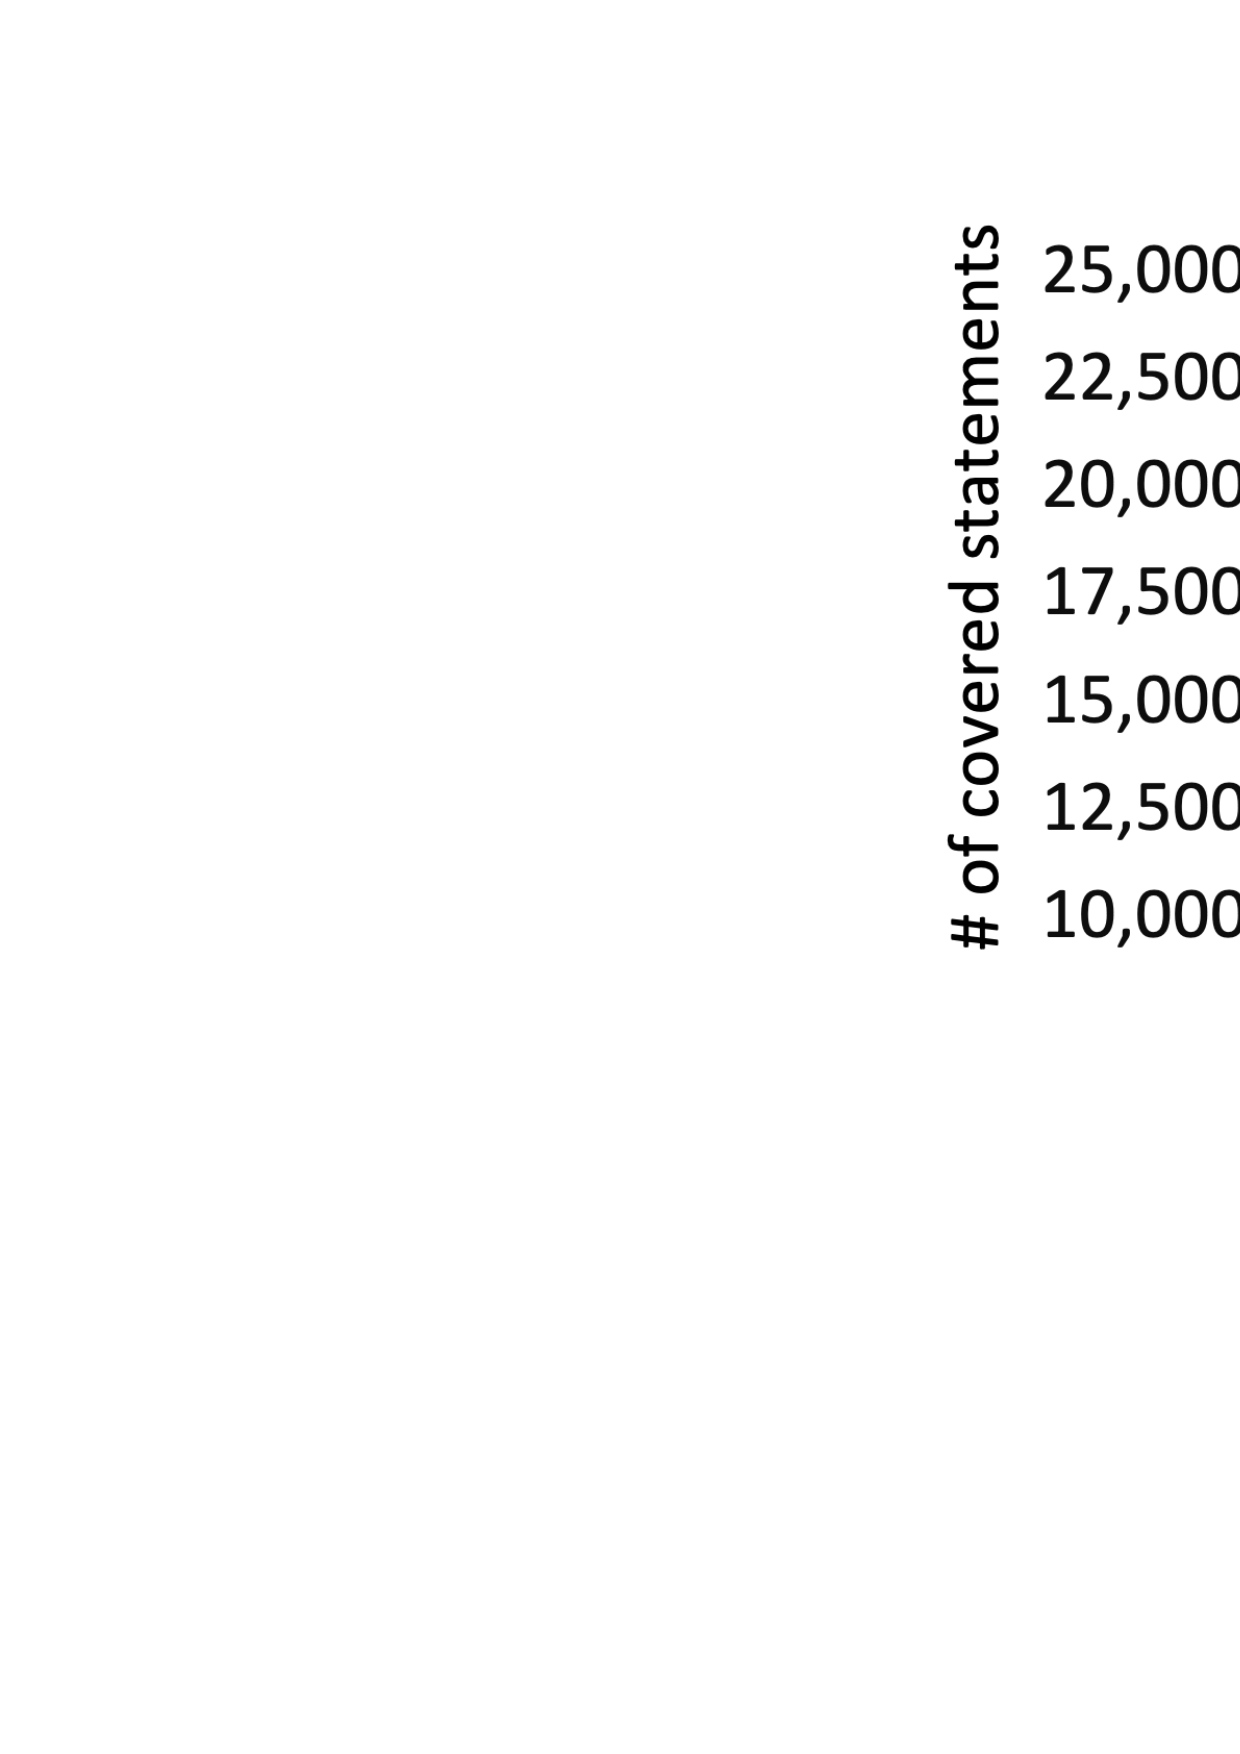
\includegraphics[width=\textwidth]{img/stmt-coverage.pdf}
    \caption{The statement coverage}
    \label{fig:stmt-coverage}
  \end{subfigure}
  \quad
  \begin{subfigure}[t]{0.48\textwidth}
    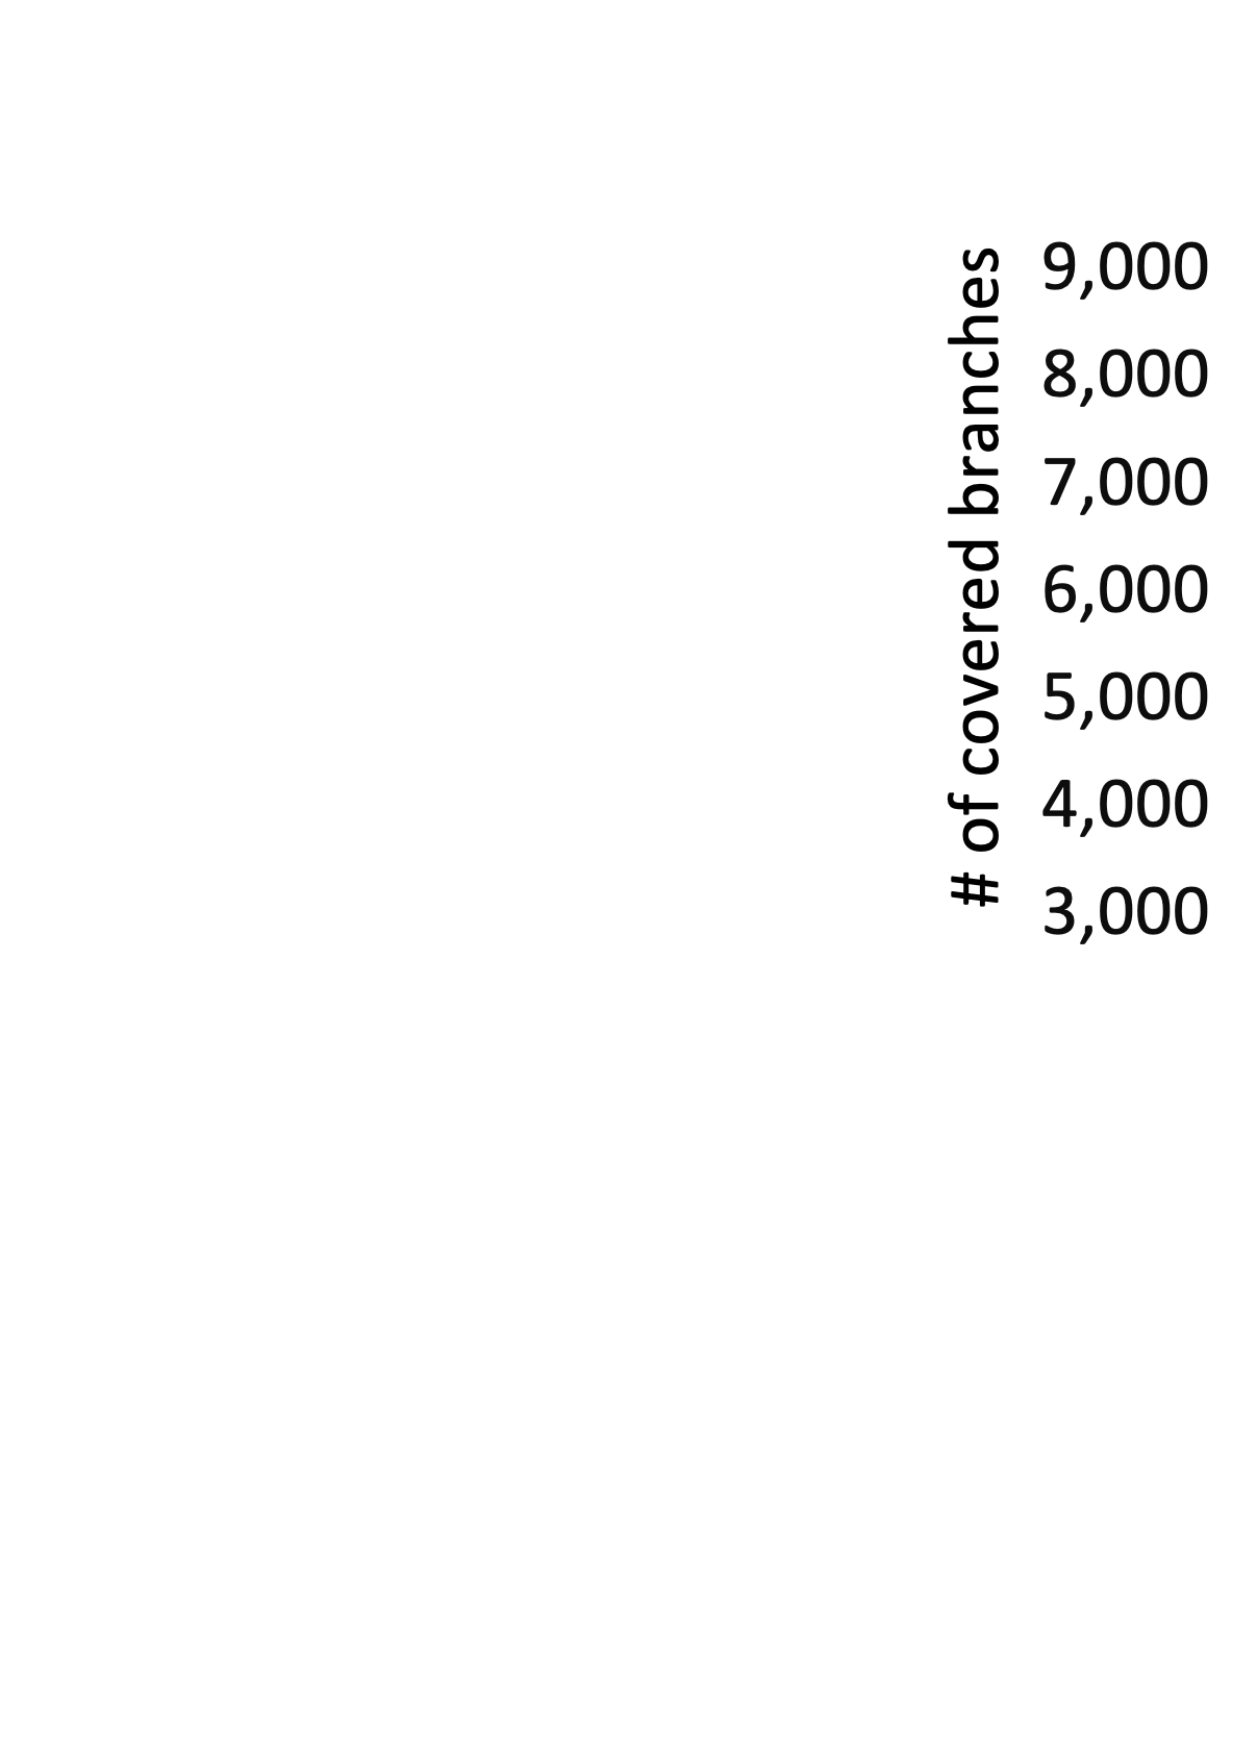
\includegraphics[width=\textwidth]{img/branch-coverage.pdf}
    \caption{The branch coverage}
    \label{fig:branch-coverage}
  \end{subfigure}
  \caption{The semantics coverage changes during the test generation phase}
  \label{fig:sem-coverage}
  \vspace*{-1em}
\end{figure*}

To evaluate $\tool$ that performs the $N$+1-differential testing of JavaScript
engines and specification, we applied our tool to four JavaScript engines that
fully support modern JavaScript features and the most recent specification,
ECMAScript 2020 (ES11, 2020).  We targeted the following four JavaScript
engines and all of them supports
ES11\footnote{https://github.com/graalvm/graaljs\#current-status}\footnote{https://bellard.org/quickjs/}\footnote{https://blog.moddable.com/blog/xs10/}\footnote{https://v8.dev/}:
\begin{itemize}
  \item \textbf{GraalJS(v20.1.0):} A JavaScript implementation built on
    GraalVM\cite{graaljs}, which is a Java Virtual Machine (JVM) based on
    HotSpot/OpenJDK developed by Oracle.
  \item \textbf{QuickJS(2020-04-12):} A small and embedded JavaScript engine developed by
    Fabrice Bellard and Charlie Gordon\cite{qjs}.
  \item \textbf{Moddable XS(v10.2.1):} A JavaScript engine at the center of the Moddable
    SDK\cite{xs}, which is a combination of development tools and runtime
    software to create applications for microcontrollers.
  \item \textbf{V8(v8.5):} The Google's open source high-performance JavaScript and
    WebAssembly engine\cite{v8}, written in C++.
\end{itemize}
To extract mechanized specification from ECMAScript, we utilize the tool
$\jiset$, which is a JavaScript IR-based semantics extraction toolchain.
automatically extracted from a given ECMAScript.  To focus on the semantics of
core JavaScript semantics, we only consider the semantics of strict mode
JavaScript codes that pass syntax checking including the EarlyError rules.  To
filter out the JavaScript codes that are not strict or fail the syntax checking,
we utilize the syntax checker of the most reliable JavaScript engine, V8.
We performed our experiments on a machine equipped with 4.0GHz Intel(R) Core(TM)
i7-6700k and 32GB of RAM (Samsung DDR4 2133MHz 8GB*4).  We evaluated our tool
based on the following four research questions:
\begin{itemize}
  \item {\bf RQ1 (Coverage of Generated Tests)} The semantics coverage compared
    to Test262, the manually written official conformance test suite for
    ECMAScript.
  \item {\bf RQ2 (Bug Detection in JavaScript Engines)} The number of bugs in
    four JavaScript engines detected by $\tool$.
  \item {\bf RQ3 (Bug Detection in ECMAScript)} The number of specification bugs
    in ES11 detected by $\tool$.
\end{itemize}


\subsection{Coverage of Generated Tests}

For the first step, we synthesize seed programs via \textsf{Seed Synthesizer}
based on the syntax of ES11.  It synthesizes \inred{1,112} JavaScript programs
in about \inred{10} seconds and covers \inred{97.25\% (395/406)} of reachable
alternatives in syntax productions.  The seed programs becomes the initial
program pool and it gradually grows via \textsf{Target Selector} and
\textsf{Program Mutator}.  Figure~\ref{fig:sem-coverage} shows the change of
semantics coverage of the program pool during the iterative process in
\inred{45} hours.  The left and right graphs show the statement and branch
coverages, respectively.  The red line for each graph denotes the coverage of
tests of Test262.  For the statement coverage, \inred{29,728} statements exist
in ES11 and tests in Test262 covers \inred{22,425 (75.43\%)} statements.  The
initial program pool covers \inred{12,766 (42.94\%)} statements and the final
program pool covers \inred{21,249 (71.48\%)} statements.  For branch coverage,
\inred{11,448} branches exist in ES11 and tests in Test262 covers \inred{7,944
(69.39\%)} branches.  The initial program pool covers \inred{3,986 (34.82\%)}
branches and the final program pool covers \inred{7,476 (65.30\%)} branches.

\begin{table}
  \caption{The number of successes and covered branches for mutation methods}
  \label{table:mutation-method}
  \vspace*{-1em}
  \small
  \[
    \begin{array}{l?r|r}
      \telembf{c?}{Mutation Methods}      & \telembf{c|}{Success} & \telembf{c}{Branch (Avg.)}\\\toprule\\[-1.4em]
      \text{Nearest Syntax Tree Mutation} & \rtext{436}           & \rtext{1,450 (3.33)}\\\hline
      \text{Random Mutation}              & \rtext{320}           & \rtext{910   (2.84)}\\\hline
      \text{Statement Insertion}          & \rtext{201}           & \rtext{672   (3.34)}\\\hline
      \text{Object Substitution}          & \rtext{162}           & \rtext{453   (2.80)}\\\hline
      \text{String Substitution}          & \rtext{4}             & \rtext{5     (1.25)}\\\hline
      \hline
      \telembf{c?}{Total}                 & \rtext{1,123}         & \rtext{3,490 (3.11)}\\
    \end{array}
  \]
  \vspace*{-1.5em}
\end{table}

Table~\ref{table:mutation-method} shows the number of successes and covered
branches for each mutation method during the test generation phase. In total,
$\tool$ succeeds to synthesize \inred{1,123} programs that covers \inred{3,490}
more branches than the initial program pool.  Among five mutation methods, the
nearest syntax tree mutation is the most contributed method (\inred{436}
successes and \inred{1,450} covered branches) and the least one is the string
substitution (\inred{4} successes and \inred{5} covered branches).  On average,
\inred{3.11} branches are covered by one successful mutation.

Finally, $\tool$ generates \inred{X,XXX} JavaScript programs and the average
length of generated programs is \inred{XX.XX}.  After injecting asseritons by
\textsf{Asseriton Injector}, generated programs become conformance tests and
their average length is \inred{XXX.XX}.  Compared to Test262, the number of
generated tests are much smaller and their sizes also shorter than that of tests
in Test262.  Test262 provides \inred{XX,XXX} tests for the same range of
semantics and their average size is \inred{XXX.XX}.


\subsection{Bug Detection in JavaScript Engines}

We introduced six different kinds of assertions used in \textsf{Asseriton
Injector}: exceptions (\textsf{Exc}), variable values (\textsf{Var}), object
values (\textsf{Obj}), property descriptors (\textsf{Desc}), property orders
(\textsf{Ord}), and internal methods and slots (\textsf{In}).

\begin{table}
  \caption{The number of engine bugs detected by $\tool$}
  \label{table:engine-bug}
  \vspace*{-1em}
  \small
  \[
    \begin{array}{l?r|r|r|r|r|r?r}
      \telembf{c?}{Engines} &
      \telemsf{c|}{Exc} &
      \telemsf{c|}{Var} &
      \telemsf{c|}{Obj} &
      \telemsf{c|}{Desc} &
      \telemsf{c|}{Ord} &
      \telemsf{c?}{In} &
      \telembf{c}{Total}\\\toprule\\[-1.4em]

      \text{GraalJS}      & \inred{0} & \inred{0} & \inred{0} & \inred{0} & \inred{0} & \inred{0} & \inred{0}\\\hline
      \text{QuickJS}      & \inred{0} & \inred{0} & \inred{0} & \inred{0} & \inred{0} & \inred{0} & \inred{0}\\\hline
      \text{Moddable XS}  & \inred{0} & \inred{0} & \inred{0} & \inred{0} & \inred{0} & \inred{0} & \inred{0}\\\hline
      \text{V8}           & \inred{0} & \inred{0} & \inred{0} & \inred{0} & \inred{0} & \inred{0} & \inred{0}\\\hline
      \hline
      \telembf{c?}{Total} & \inred{0} & \inred{0} & \inred{0} & \inred{0} & \inred{0} & \inred{0} & \inred{0}
    \end{array}
  \]
  \vspace*{-1.5em}
\end{table}


\subsection{Bug Detection in ECMAScript}

\begin{table*}[t]
  \centering
  \caption{Specification bugs in ECMAScript 2020 (ES11) detected by $\tool$}
  \label{table:spec-bug}
  \vspace*{-.5em}
  \small
  \begin{tabular}{c?l|c|c|c|r|r}
    \telembf{c?}{\bf Name} &
    \telembf{c}{\bf Description} &
    \telembf{c}{\bf Lang} &
    \telembf{c}{\bf Created} &
    \telembf{c}{\bf Resolved} &
    \telembf{c}{\bf Existed} &
    \telembf{c}{\bf \# Fails} \\\toprule\\[-1.4em]

    ES11-1 &
    \makecell[l]{} &
    \inred{O} &
    \inred{XXXX-XX-XX} &
    \inred{XXXX-XX-XX} &
    \inred{X,XXX} days &
    \inred{X,XXX} \\\hline

    ES11-2 &
    \makecell[l]{} &
    \inred{O} &
    \inred{XXXX-XX-XX} &
    \inred{XXXX-XX-XX} &
    \inred{X,XXX} days &
    \inred{X,XXX} \\\hline

    ES11-3 &
    \makecell[l]{} &
    \inred{O} &
    \inred{XXXX-XX-XX} &
    \inred{XXXX-XX-XX} &
    \inred{X,XXX} days &
    \inred{X,XXX} \\\hline

    ES11-4 &
    \makecell[l]{} &
    \inred{O} &
    \inred{XXXX-XX-XX} &
    \inred{XXXX-XX-XX} &
    \inred{X,XXX} days &
    \inred{X,XXX} \\\hline

    ES11-5 &
    \makecell[l]{} &
    \inred{O} &
    \inred{XXXX-XX-XX} &
    \inred{XXXX-XX-XX} &
    \inred{X,XXX} days &
    \inred{X,XXX} \\\hline

    ES11-6 &
    \makecell[l]{} &
    \inred{O} &
    \inred{XXXX-XX-XX} &
    \inred{XXXX-XX-XX} &
    \inred{X,XXX} days &
    \inred{X,XXX} \\\hline

    ES11-7 &
    \makecell[l]{} &
    \inred{O} &
    \inred{XXXX-XX-XX} &
    \inred{XXXX-XX-XX} &
    \inred{X,XXX} days &
    \inred{X,XXX}
  \end{tabular}
\end{table*}

\inred{TODO}

\section{Related Work}\label{sec:related}
\inred{TODO}

\begin{itemize}
  \item CodeAlchemist\cite{codealchemist}
  \item Csmith\cite{csmith}
  \item Grammar-based Whitebox Fuzzing\cite{grammar-whitebox}
  \item Montage\cite{montage}
  \item QuickCheck\cite{quickcheck}
  \item SAGE\cite{sage}
  \item Rnadom String from a CFG\cite{cfg-gen}
  \item N-version Testing for Lifter\cite{ir-diff-test}
  \item NEZHA\cite{nezha}
  \item JavaScript History\cite{js-hopl}

\end{itemize}

\section{Conclusion}\label{sec:conclude}
The development of modern languages follow continuous integration (CI) and
continuous deployment (CD) approach to instantly support fast changing user
demands.  It make more difficult to find both of semantics bug in implementations
and the specification.  To alleviate this problem, we introduce
$N$+1-differential testing, which is the first technique to test both of
implementations and the specification.  We actualized our approach for the
JavaScript programming language via $\tool$, which performs $N$+1-differential
testing for modern JavaScript engines and their specification, ECMAScript.  It
automatically generated \inred{-} JavaScript programs with \inred{-}\% of syntax
coverage and \inred{-}\% of semantics coverage on the latest version of
ECMAScript (ES11, 2020).  Our tool injected assertions to them in order to
convert them as conformance tests.  We executed generated conformance tests on
four different modern JavaScript engines: GraalJS, QuickJS, Moddable XS, and V8.
Using the execution results, we found \inred{-} specification bugs and
\inred{-} engine bugs (\inred{-} for GraalJS, \inred{-} for QuickJS, \inred{-}
for Moddable XS, and \inred{-} for V8). All of them confirmed by the TC39, the
committee of ECMAScript, and authors of JavaScript engines and will be fixed.
We also localized detected bugs on ECMAScript and the average ranks of actual
bug locations are \inred{-} for algorithms and \inred{-} for algorithm steps.


\bibliographystyle{IEEEtran}
\bibliography{ref}

\end{document}
